\chapter{Software development and management processes}
The following chapter explains the software development and management processes that were employed throughout the project. In the following section some of the necessary terminology will be introduced and explained. Subsequently the process description will be given, followed by a comparison to established process models. %TODO Kanskje urdering/konklusjon

\section{Terms}
Here follows a description of terms as used in the current project.

\begin{description}

\item[Agile methods] \label{def:agile} are a set of software development methods that emphasize on adapting to change over following a predetermined plan, continuous customer collaboration over contract negotiation and implementation over documentation.

\item[Extreme programming] (XP) is an agile software development methodology which favours improving of a software and quick responses, like Iterative development except it is faster. Extreme programming uses a cycle based programming system like the Iterative approach. Unlike the Iterative approach it has a checkpoint after each stage, where the code is being released and new customer requirements is added. The customer are often intimately involved in prioritizing and specifying the requirements. Extreme programming enables the possibility to make it so that several developers can produce code, integrate and test it on the same day.  %TODO: FIX

\item[Incremental development] \label{def:incrementalDev} is an approach to software development that is "based on the idea of developing an initial implementation, exposing this to user comment and evolving it through several versions until an adequate system has been developed"\footnote{\cite{sommerville}, page 32}. Benefits to incremental development include adaptability to changing requirement and facilitation of feedback. In the negative side, it can be hard to keep an overview of the progress of the entire system, making it harder to plan ahead for deadlines.

\item[Plan-driven development] \label{def:plan-driven} is an approach to software development that recommends careful planning of the software development process, work breakdown and scheduling before starting the implementation process. 

\item[Sprint] \label{def:sprint} is the period unit in which work is planned and done. It is customary to operate with sprints of 2-4 weeks, but the current project operated with sprints of 1-2 weeks.

\item[Spike] \label{def:spike} is a sprint spent primarily or solely on non-programming activities, such as research, documentation or planning.

\item[Stand-up] \label{def:dailyScrum} is a meeting in which all the group members explain shortly what they have been doing since the last meeting, what they are planning to do until next time, and any help or advice they need to continue. Stand-ups function as a binding factor that keeps the entire group on the same page, and provides flexibility by giving the opportunity to change the plans and tasks partway through the sprint.

\end{description}

\section{Development process}
\label{def:devProcess}
The customer required an incremental development process where ideally a new version of the product could be demonstrated at every weekly customer meeting. Furthermore, plans for the following week were to be sketched in collaboration with the customer at the weekly meeting. With such short-term plans, and as the requirements were still vague and the product to be developed largely experimental, a high degree of flexibility was required. A plan-driven approach was therefore impossible at the beginning of the project. The process model employed in the early stages of development was therefore based on agile methods, and extreme programming in particular. Due to the customer requirements, sprint length was set to one week, with the possibility for two week sprints in certain cases, such as when the customer is unable to show up to a weekly meeting, or the required tasks are more extensive than usual. 

%TODO: SKILNAD noraml XP og oss

Meetings between the customer and the group normally took place on Fridays, and were followed by a group planning and work session. Stand-ups were originally planned for Wednesdays and Sundays, as these were the only times all the group members were available at the same time. The meetings at Sundays were conducted online, and the Wednesday meetings at the university. The Sunday stand-ups were abolished after a few weeks, as little work had normally been done between the Friday session and the Sunday stand-up. To compensate for the relative low frequency of stand-ups (Agile development teams in full-time work environments normally hold daily stand-ups.) other communication channels, such as e-mail and Trello\footnote{See page \pageref{def:trello} for more information} were heavily used.

After Easter several changes in the circumstances prompted a change in development methodology. These includes:
\begin{itemize}
\item A much clearer definition of the requirements and the project goals had gradually emerged. 
\item The time left until the final deadline had decreased significantly.
\item The number of potential tasks left had remained close to constant throughout the semester, as finishing one task often leads to insights as to what can be done further.
\item The group had attained a better understanding of its own work process. 
\item Significant integration and system testing was needed.
\end{itemize}
These circumstances revealed the necessity for and possibility to make concrete plans, and prioritize between the potential tasks. Therefore,  the development model was changed to a plan-driven approach that still enforced incremental delivery. Some flexibility was still maintained, by making a buffer of optional tasks in case of delays or unforeseen requirement changes. Some elements from XP were still preserved, such as pair programming and individual choice of tasks.

\subsection {How Tasks are assigned}
After WBS, tasks were uploaded to Trello. In theory, every member would pick the tasks he was most interested in, without any involvement of the group leader. However, because there were often students missing from the meetings, and these failed to choose tasks independently, the group leader was often required to assign some tasks. Tasks related to documentation were assigned by the document organizer rather than the group leader.

Communication between the group members throughout the week enabled reallocation of tasks from members that were not able to work as much as required or had gotten tasks that took longer than expected.  

\section{Meetings with Customer and Supervisor}
The main essence of the project was that it is based on the principle of the incremental working model. Thus include that the project needs regularly being updated by the stakeholding instances(customer,supervisor) for requirements and functionality. For this reason meetings between the group and the customer has to be made regularly every friday with the customer and every second monday with supervisor.   From that principles the project benefits in many aspects: - The project gains current updates - The progressing of the project is consistent - The project has the chance of getting feedback before and after the tasks are done - The project is splitted in small pieces of actionable specific smaller tasks - This smaller elements can be discussed in way being realistic or not quite before they are started - Due to the smaller pieces progress and mistakes can be backtracked - A way of working close for satisfying the customer - The group can react when the supervisor or customer are not understanding the interim results.


\section{Plans}

Nearing the end of every sprint, the customer and group agreed upon the content of the following sprint. This list has been placed in Figure \ref{tab:sprintList}, and provided a short summary of what was accomplished in a particular time-frame. 


\section{Team Roles and Organization}
\subsection{The group} \label{def:the group}
There was not much place for specific roles among the group, as it was a small group, and the project required that all the members were capable and willing to work at all the tasks. This makes a difference from development models with specific roles and tasks assigned. Roles that were set for the group were therefore mainly organizers, so that one person was to keep awareness of what work needed to be completed in a particular domain, and share it with the rest of the group:

\begin{description}

\item[Group Leader] Elias was made organizer, and got the responsibilities of reminding the group of what to do.
\item[Document-organizer] Johannes was tasked with organizing documentation and distributing the work of writing the report to the group. 
\end{description}
 
 Otherwise the group had no codified responsibilities, and as all the team members were roughly equally experienced at the start, team members were not constantly assigned particular tasks.
 

\section{Comparison}
The development model used by the group was a form of agile development. Other well-known examples of agile methodologies are Scrum and Extreme Programming.
 
\section{Work Breakdown Structure}
With a development methodology that stresses short term goals, it is only possible to plan WBS for the current period. After the customer has specified the goal for the following week, we immediately sat down and defined the WBS for the given period. This was, a WBS was developed incrementally by adjoining the new WBS to the previous. The WBS was made in graphical form, as can be seen in Figure \ref{fig:WBS}.

\begin{figure}[p]

\setlength\fboxsep{0pt}
\setlength\fboxrule{1pt}\noindent\makebox[\textwidth]{%
 \fbox{
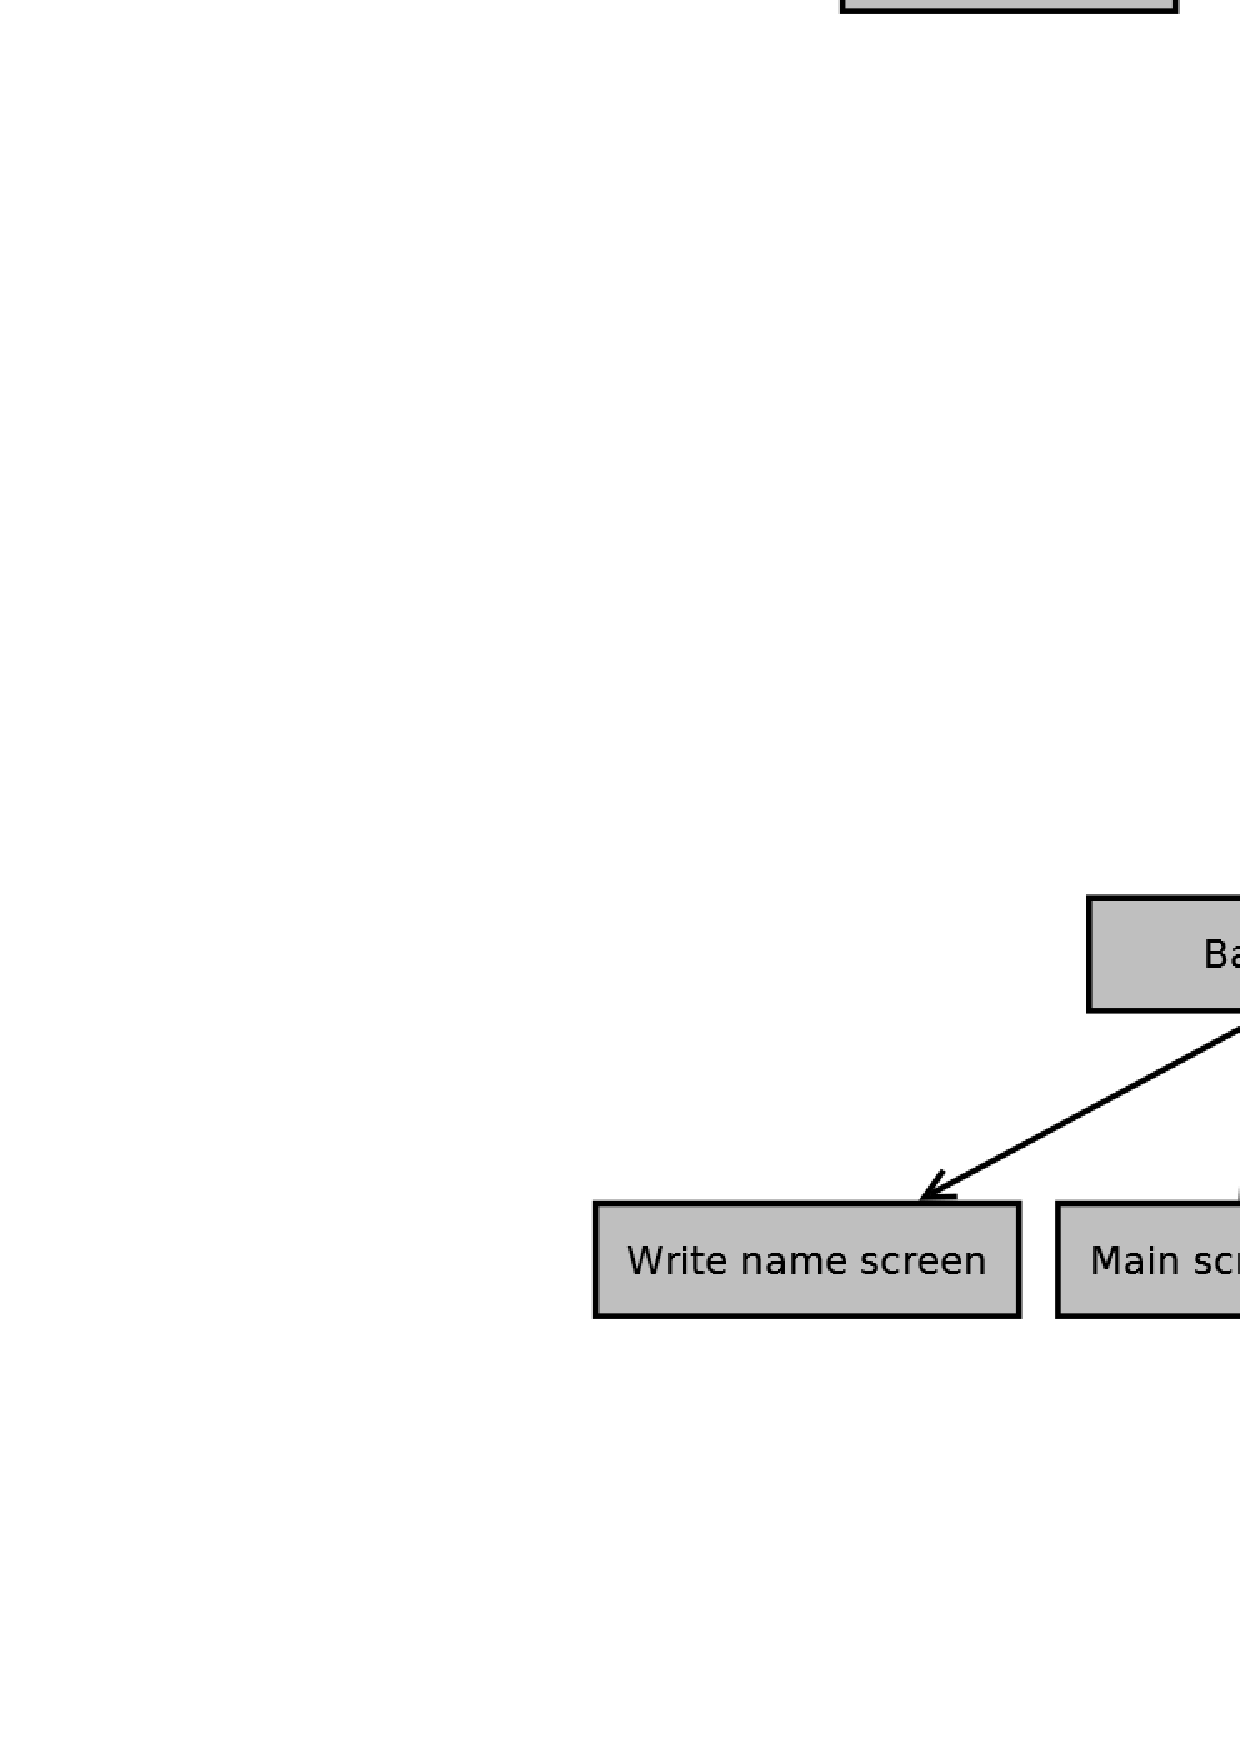
\includegraphics[width=1.45\textwidth , angle=270]{Res/WBS15313.png}
}
}

\caption{The final WBS}
\label{fig:WBS}
\end{figure}
